\documentclass[english,notitlepage,letterpaper, 10pt]{article} % para articulo en castellano
\usepackage{cite}
\usepackage[utf8]{inputenc} % Acepta caracteres en castellano
\usepackage[english]{babel} % silabea palabras castellanas
\usepackage{amsmath}

\usepackage{amsfonts}
\usepackage{amssymb}
\usepackage{hyperref} % navega por el doc
\usepackage{graphicx}
\usepackage{geometry}      % See geometry.pdf to learn the layout options.
\geometry{letterpaper}                   % ... or a4paper or a5paper or ... 
%\geometry{landscape}                % Activate for for rotated page geometry
%\usepackage[parfill]{parskip}    % Activate to begin paragraphs with an empty line rather than an indent
\usepackage{epstopdf}
\usepackage{fancyhdr} % encabezados y pies de pg

\usepackage{listings}
\usepackage{color}

\definecolor{dkgreen}{rgb}{0,0.6,0}
\definecolor{gray}{rgb}{0.5,0.5,0.5}
\definecolor{mauve}{rgb}{0.58,0,0.82}

\lstset{frame=shadowbox,
  language=Matlab,
  aboveskip=3mm,
  belowskip=3mm,
  showstringspaces=false,
  columns=flexible,
  basicstyle={\small\ttfamily},
  numbers=left,
  numberstyle=\tiny\color{gray},
  keywordstyle=\color{blue},
  commentstyle=\color{dkgreen},
  stringstyle=\color{mauve},
  breaklines=true,
  breakatwhitespace=true
  tabsize=3
  rulesepcolor=\color{blue}
}

\newcommand{\university}{\normalsize Universidad Industrial de Santander}
\newcommand{\faculty}{\normalsize  Escuela de Ingenier\'ia de Sistemas e Inform\'atica}
\newcommand{\codigo}{\normalsize  XXXXX}
\newcommand{\grupo}{\normalsize  XX}
\pagestyle{fancy} 
\chead{\bfseries Lab. } 
\lhead{} % si se omite coloca el nombre de la seccion
\rhead{\today} 
\lfoot{\it  An\'alisis N\'umerico } 
\cfoot{\university} 
\rfoot{\thepage} 

\voffset = -0.25in 
\textwidth = 7.5in
\textheight = 9in
\oddsidemargin = -0.5in
\headheight = 20pt 
\headwidth = 7.5in
\renewcommand{\headrulewidth}{0.5pt}
\renewcommand{\footrulewidth}{0,5pt}
\DeclareGraphicsRule{.tif}{png}{.png}{`convert #1 `dirname #1`/`basename #1 .tif`.png}


\begin{document}

\title{	\vspace{-12mm}
\includegraphics[width=0.2\linewidth]{Logos/UIS.pdf}\\Informe Laboratorio: An\'alisis Num\'erico\\  \centering Pr\'actica No. X}
\author{
\textbf{Nombre Apellido:} \\ \textbf{C\'odigo:} \codigo\\
\textbf{Grupo:} \grupo\\
\textit{\faculty}\\
\textit{\university}}
\date{\today}
\maketitle

\section{Introducci\'on}
Incluya una breve descripci\'on del informe de laboratorio \cite{ejemplo}. 

\section{Desarrollo}

\begin{enumerate}
	\item Ejemplo de numeraci\'on. En la Fig. \ref{Figura4}, se presenta un ejemplo para incluir figuras.
	\begin{enumerate}
	\item Ejemplo de numeraci\'on.
			
			\begin{figure}[!h]
				\begin{center}
					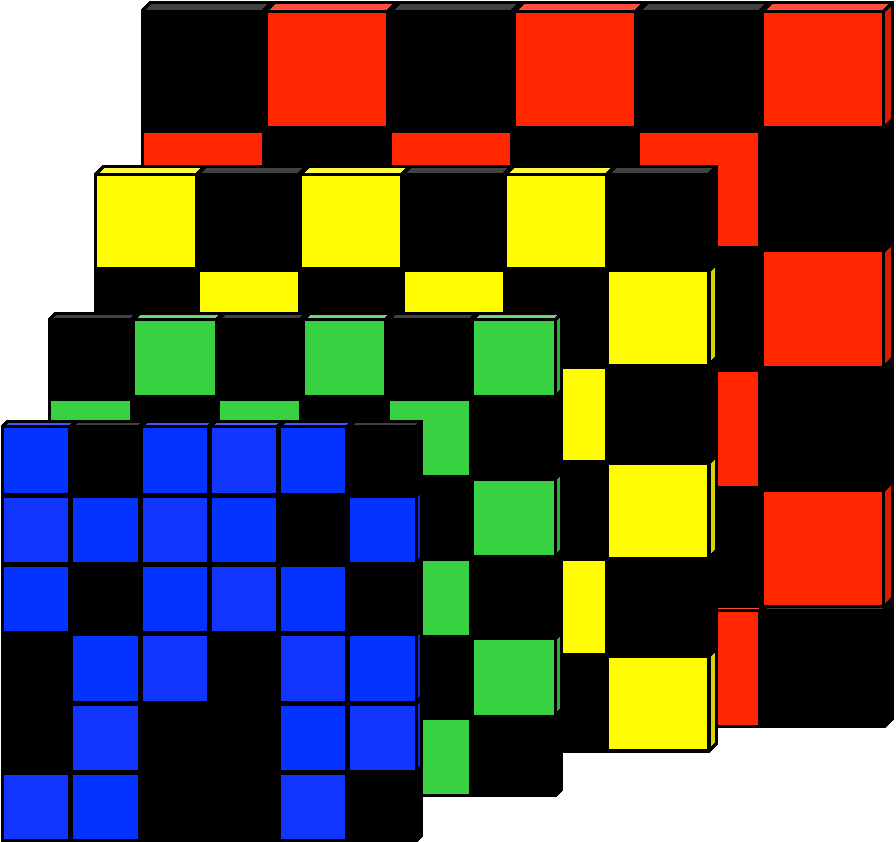
\includegraphics[width=1.0in]{Images/imagen1.pdf}
					\caption{Ejemplo figura.}
					\label{Figura4}
				\end{center}
			\end{figure}

	\end{enumerate}

\end{enumerate}
\newpage
\section{Anexos}
En los anexos puede incluir el c\'odigo de Matlab.

\begin{lstlisting} 
hyperimg(:,:,1) = imread('Fig1138(a)(WashingtonDC_Band1_564).tif');
hyperimg(:,:,2) = imread('Fig1138(b)(WashingtonDC_Band2_564).tif');
hyperimg(:,:,5) = imread('Fig1138(e)(WashingtonDC_Band5_564).tif');
\end{lstlisting}


\bibliographystyle{ieeetr}
\bibliography{biblio}





\end{document}  


